% paper/sections/05_analysis.tex
\section{Analysis and Ablations}
\label{sec:ablations}

\begin{figure}[h]
\centering
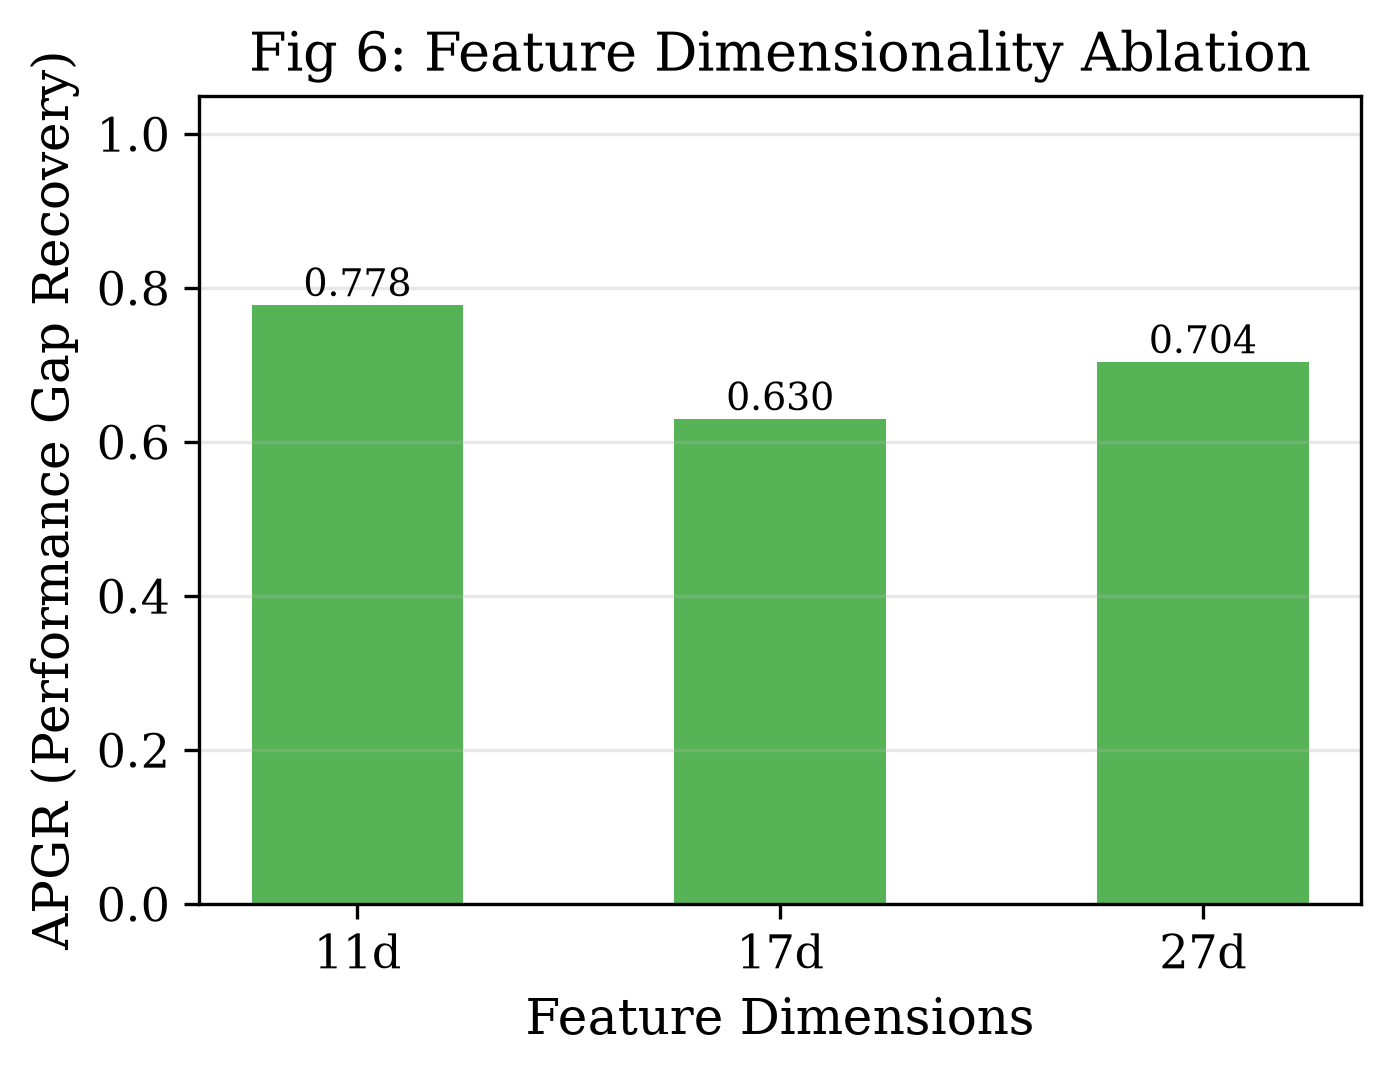
\includegraphics[width=0.32\linewidth]{figures/fig6_feature_dim_ablation.png}
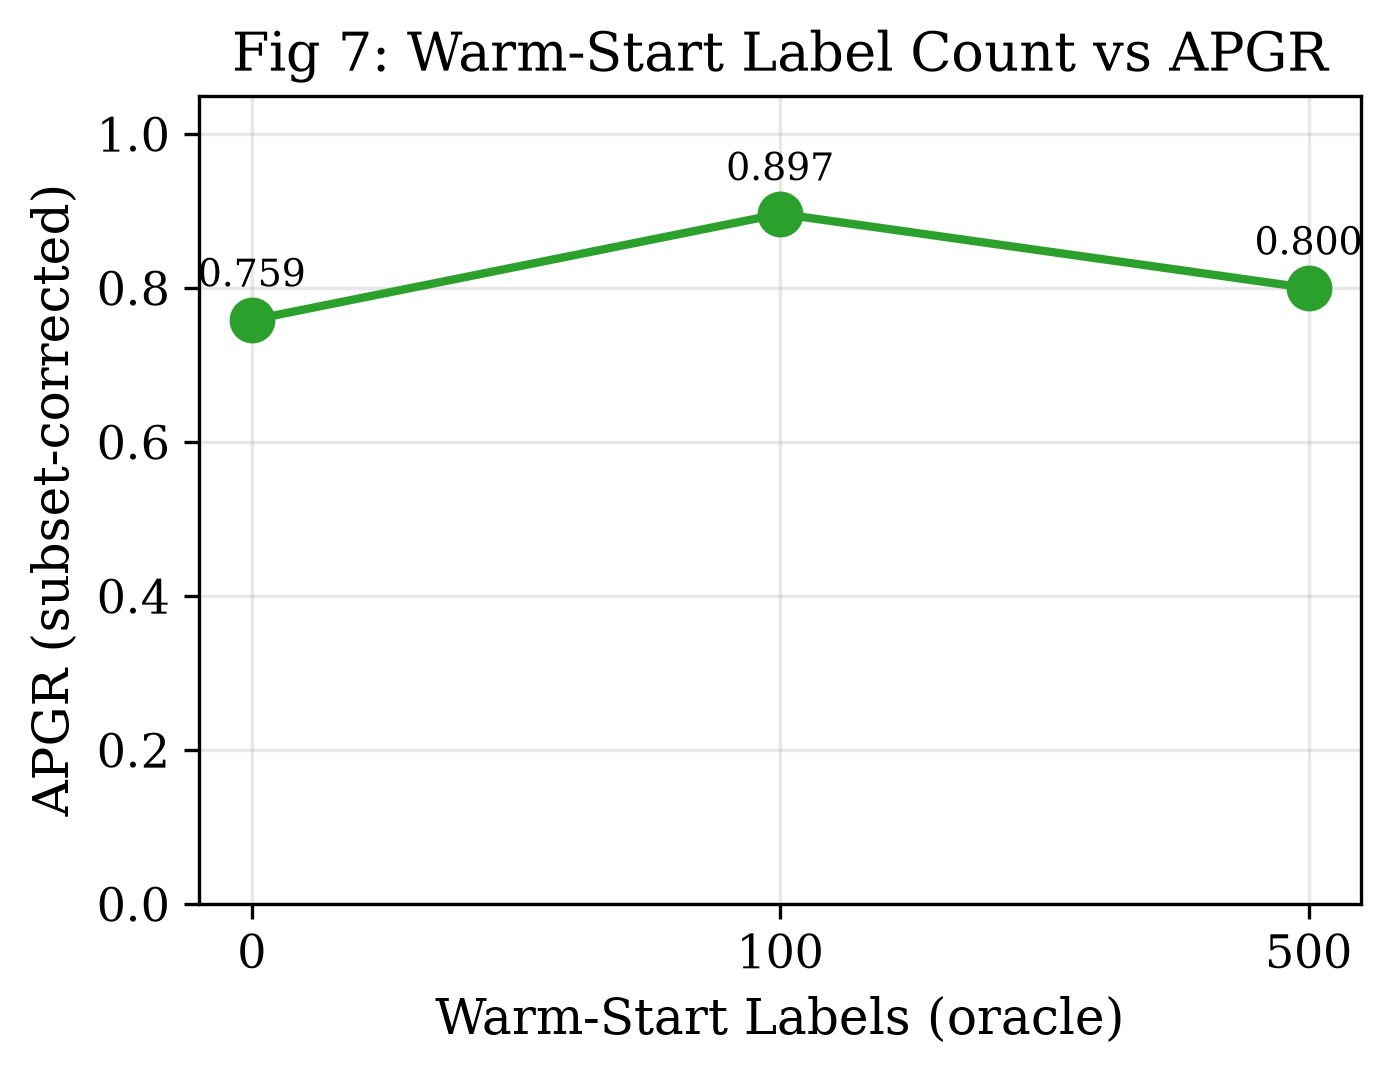
\includegraphics[width=0.32\linewidth]{figures/fig7_warm_start_ablation.png}
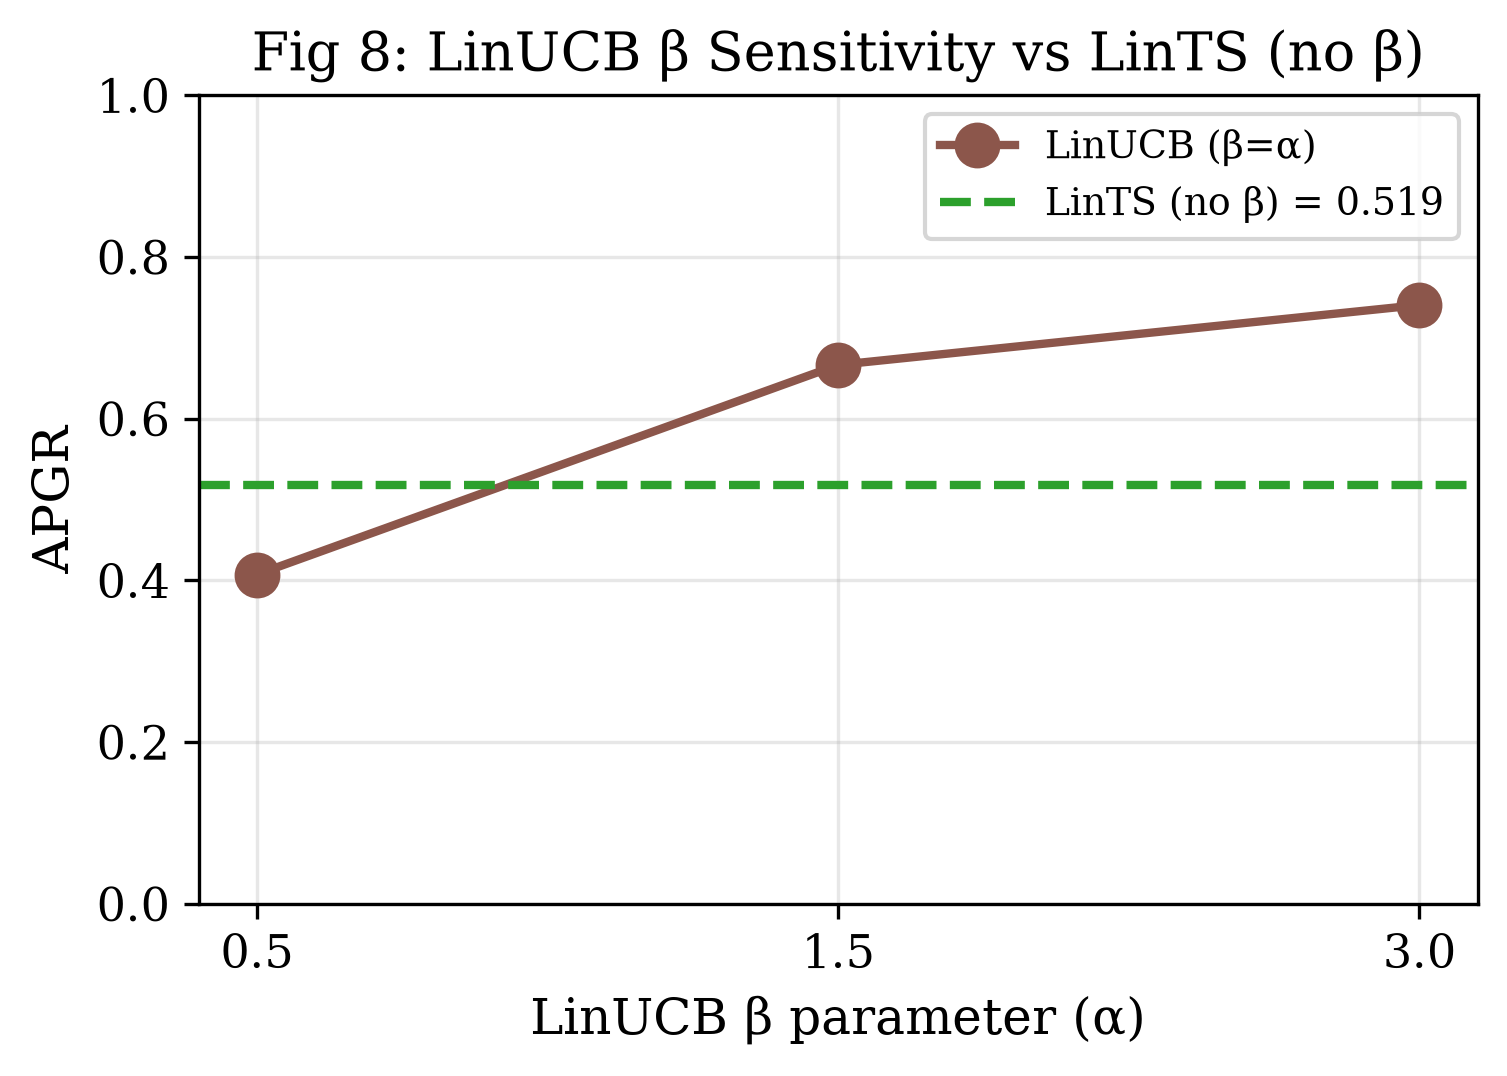
\includegraphics[width=0.32\linewidth]{figures/fig8_beta_sensitivity.png}
\caption{Left: Feature dimensionality ablation. Center: Warm-start labels vs APGR. Right: LinUCB $\beta$ sensitivity vs LinTS.}
\end{figure}

\subsection{Feature Dimensionality}

We compare LinTS variants using 11, 17, and 27 feature dimensions (zero-padding to 27d).
Results on MMLU (seed=42): 11d achieves APGR=0.778, 17d achieves APGR=0.630, and 27d achieves APGR=0.704.
The non-monotonic trend (11d $>$ 27d $>$ 17d) is unexpected and warrants cautious interpretation.
One hypothesis is that the 6 extended keyword features (indices 11--16) introduce noise for MMLU's multiple-choice format, while the zero-padded model-feature dimensions (17--26) in the 27d variant reduce the effective weight of the noisy features, partially recovering performance.
However, alternative explanations are equally plausible: the single seed (42) may be insufficient for stable estimates, the L2-normalization may interact with dimensionality in ways that confound the comparison, or the feature space may benefit from more deliberate engineering rather than simple dimension reduction.
We report this as an exploratory result and recommend multi-seed validation before drawing conclusions about optimal feature dimensionality.

\subsection{Warm-Start Labels}

We initialize LinTS with 0, 100, or 500 oracle labels (always reward arm~1, the strong model) before online evaluation on the remaining 100 queries.
Using subset-corrected baselines (strong/weak accuracy recomputed on the same 100 eval queries to avoid data leakage), APGR improves from 0.759 (cold start on subset, higher than the full-set 0.593 due to different query composition) to 0.897 (100 labels) and 0.800 (500 labels).
The non-monotonic improvement — 100 labels outperforms 500 — arises because 500 oracle labels strongly bias the posterior toward the strong arm, reducing exploration on the remaining 100 eval queries.
Even 100 warm-start labels substantially reduce cold-start regret, suggesting that a small labeled calibration set is beneficial when available.

\subsection{LinUCB $\beta$ Sensitivity vs LinTS}

LinUCB APGR at $\beta \in \{0.5, 1.5, 3.0\}$: 0.407, 0.667, 0.741 respectively.
Higher $\beta$ encourages more exploration, routing more queries to the strong arm, and increases APGR at the cost of higher API spend.
LinTS (no $\beta$) achieves APGR=0.519, falling between $\beta=0.5$ and $\beta=1.5$ without any hyperparameter tuning.
This confirms that LinTS provides parameter-free uncertainty quantification via posterior sampling, making it preferable in deployment settings where calibration is impractical.

\subsection{Distribution Shift}

LinTS-27d trained and evaluated on GSM8K achieves 92.5\%$\pm$0.4\% (APGR=0.153 using GSM8K baselines: strong=97.3\%, weak=91.7\%).
This is notably higher than TS-Cat (91.1\%, APGR=$-0.106$), showing that the 27-dim feature representation provides meaningful routing signal on math problems beyond simple category-level preferences.
The lower APGR on GSM8K relative to MMLU reflects the harder problem: GSM8K's strong/weak accuracy gap is only 5.6 percentage points (vs. 4.5 on MMLU), and math-specific keyword features provide limited discriminative signal for mathematical reasoning tasks.
Cross-task generalization (MMLU-trained $\rightarrow$ GSM8K evaluation) is left to future work.

\subsection{Reproducibility}

All results in this paper are from real API calls with fixed random seeds, ensuring full reproducibility.
Experiment scripts, configurations, and random seeds are provided in the supplementary material.

\textbf{RouteLLM-SW note:} The SW router uses \texttt{all-MiniLM-L6-v2} (384-dim) as the embedding model, as OpenRouter does not expose the original \texttt{text-embedding-3-small} arena embeddings. Win-rate scores cluster at 0.218--0.233 on both MMLU and GSM8K (below all thresholds), reflecting domain mismatch between Chatbot Arena conversational queries and structured benchmarks. The degraded embedding model is an additional confound; results should not be interpreted as a claim that LinTS outperforms RouteLLM-SW in its native embedding configuration.
